% Options for packages loaded elsewhere
\PassOptionsToPackage{unicode}{hyperref}
\PassOptionsToPackage{hyphens}{url}
%
\documentclass[
  ,man,floatsintext]{apa6}
\usepackage{amsmath,amssymb}
\usepackage{iftex}
\ifPDFTeX
  \usepackage[T1]{fontenc}
  \usepackage[utf8]{inputenc}
  \usepackage{textcomp} % provide euro and other symbols
\else % if luatex or xetex
  \usepackage{unicode-math} % this also loads fontspec
  \defaultfontfeatures{Scale=MatchLowercase}
  \defaultfontfeatures[\rmfamily]{Ligatures=TeX,Scale=1}
\fi
\usepackage{lmodern}
\ifPDFTeX\else
  % xetex/luatex font selection
\fi
% Use upquote if available, for straight quotes in verbatim environments
\IfFileExists{upquote.sty}{\usepackage{upquote}}{}
\IfFileExists{microtype.sty}{% use microtype if available
  \usepackage[]{microtype}
  \UseMicrotypeSet[protrusion]{basicmath} % disable protrusion for tt fonts
}{}
\makeatletter
\@ifundefined{KOMAClassName}{% if non-KOMA class
  \IfFileExists{parskip.sty}{%
    \usepackage{parskip}
  }{% else
    \setlength{\parindent}{0pt}
    \setlength{\parskip}{6pt plus 2pt minus 1pt}}
}{% if KOMA class
  \KOMAoptions{parskip=half}}
\makeatother
\usepackage{xcolor}
\usepackage{graphicx}
\makeatletter
\def\maxwidth{\ifdim\Gin@nat@width>\linewidth\linewidth\else\Gin@nat@width\fi}
\def\maxheight{\ifdim\Gin@nat@height>\textheight\textheight\else\Gin@nat@height\fi}
\makeatother
% Scale images if necessary, so that they will not overflow the page
% margins by default, and it is still possible to overwrite the defaults
% using explicit options in \includegraphics[width, height, ...]{}
\setkeys{Gin}{width=\maxwidth,height=\maxheight,keepaspectratio}
% Set default figure placement to htbp
\makeatletter
\def\fps@figure{htbp}
\makeatother
\setlength{\emergencystretch}{3em} % prevent overfull lines
\providecommand{\tightlist}{%
  \setlength{\itemsep}{0pt}\setlength{\parskip}{0pt}}
\setcounter{secnumdepth}{-\maxdimen} % remove section numbering
% Make \paragraph and \subparagraph free-standing
\ifx\paragraph\undefined\else
  \let\oldparagraph\paragraph
  \renewcommand{\paragraph}[1]{\oldparagraph{#1}\mbox{}}
\fi
\ifx\subparagraph\undefined\else
  \let\oldsubparagraph\subparagraph
  \renewcommand{\subparagraph}[1]{\oldsubparagraph{#1}\mbox{}}
\fi
\newlength{\cslhangindent}
\setlength{\cslhangindent}{1.5em}
\newlength{\csllabelwidth}
\setlength{\csllabelwidth}{3em}
\newlength{\cslentryspacingunit} % times entry-spacing
\setlength{\cslentryspacingunit}{\parskip}
\newenvironment{CSLReferences}[2] % #1 hanging-ident, #2 entry spacing
 {% don't indent paragraphs
  \setlength{\parindent}{0pt}
  % turn on hanging indent if param 1 is 1
  \ifodd #1
  \let\oldpar\par
  \def\par{\hangindent=\cslhangindent\oldpar}
  \fi
  % set entry spacing
  \setlength{\parskip}{#2\cslentryspacingunit}
 }%
 {}
\usepackage{calc}
\newcommand{\CSLBlock}[1]{#1\hfill\break}
\newcommand{\CSLLeftMargin}[1]{\parbox[t]{\csllabelwidth}{#1}}
\newcommand{\CSLRightInline}[1]{\parbox[t]{\linewidth - \csllabelwidth}{#1}\break}
\newcommand{\CSLIndent}[1]{\hspace{\cslhangindent}#1}
\ifLuaTeX
\usepackage[bidi=basic]{babel}
\else
\usepackage[bidi=default]{babel}
\fi
\babelprovide[main,import]{english}
% get rid of language-specific shorthands (see #6817):
\let\LanguageShortHands\languageshorthands
\def\languageshorthands#1{}
% Manuscript styling
\usepackage{upgreek}
\captionsetup{font=singlespacing,justification=justified}

% Table formatting
\usepackage{longtable}
\usepackage{lscape}
% \usepackage[counterclockwise]{rotating}   % Landscape page setup for large tables
\usepackage{multirow}		% Table styling
\usepackage{tabularx}		% Control Column width
\usepackage[flushleft]{threeparttable}	% Allows for three part tables with a specified notes section
\usepackage{threeparttablex}            % Lets threeparttable work with longtable

% Create new environments so endfloat can handle them
% \newenvironment{ltable}
%   {\begin{landscape}\centering\begin{threeparttable}}
%   {\end{threeparttable}\end{landscape}}
\newenvironment{lltable}{\begin{landscape}\centering\begin{ThreePartTable}}{\end{ThreePartTable}\end{landscape}}

% Enables adjusting longtable caption width to table width
% Solution found at http://golatex.de/longtable-mit-caption-so-breit-wie-die-tabelle-t15767.html
\makeatletter
\newcommand\LastLTentrywidth{1em}
\newlength\longtablewidth
\setlength{\longtablewidth}{1in}
\newcommand{\getlongtablewidth}{\begingroup \ifcsname LT@\roman{LT@tables}\endcsname \global\longtablewidth=0pt \renewcommand{\LT@entry}[2]{\global\advance\longtablewidth by ##2\relax\gdef\LastLTentrywidth{##2}}\@nameuse{LT@\roman{LT@tables}} \fi \endgroup}

% \setlength{\parindent}{0.5in}
% \setlength{\parskip}{0pt plus 0pt minus 0pt}

% Overwrite redefinition of paragraph and subparagraph by the default LaTeX template
% See https://github.com/crsh/papaja/issues/292
\makeatletter
\renewcommand{\paragraph}{\@startsection{paragraph}{4}{\parindent}%
  {0\baselineskip \@plus 0.2ex \@minus 0.2ex}%
  {-1em}%
  {\normalfont\normalsize\bfseries\itshape\typesectitle}}

\renewcommand{\subparagraph}[1]{\@startsection{subparagraph}{5}{1em}%
  {0\baselineskip \@plus 0.2ex \@minus 0.2ex}%
  {-\z@\relax}%
  {\normalfont\normalsize\itshape\hspace{\parindent}{#1}\textit{\addperi}}{\relax}}
\makeatother

\makeatletter
\usepackage{etoolbox}
\patchcmd{\maketitle}
  {\section{\normalfont\normalsize\abstractname}}
  {\section*{\normalfont\normalsize\abstractname}}
  {}{\typeout{Failed to patch abstract.}}
\patchcmd{\maketitle}
  {\section{\protect\normalfont{\@title}}}
  {\section*{\protect\normalfont{\@title}}}
  {}{\typeout{Failed to patch title.}}
\makeatother

\usepackage{xpatch}
\makeatletter
\xapptocmd\appendix
  {\xapptocmd\section
    {\addcontentsline{toc}{section}{\appendixname\ifoneappendix\else~\theappendix\fi\\: #1}}
    {}{\InnerPatchFailed}%
  }
{}{\PatchFailed}
\keywords{infant-directed speech; reproducibility; Africa; infants; generalizability\newline\indent Word count: XYZ}
\usepackage{lineno}

\linenumbers
\usepackage{csquotes}
\usepackage{tabularx}
\usepackage{booktabs}
\usepackage{amsmath}
\renewcommand{\topfraction}{1}
\renewcommand{\bottomfraction}{1}
\renewcommand{\textfraction}{.1}
\renewcommand{\floatpagefraction}{1}
\setcounter{topnumber}{9}
\setcounter{bottomnumber}{9}
\setcounter{totalnumber}{20}
\setcounter{dbltopnumber}{9}
\PassOptionsToPackage{english}{babel}
\usepackage{babel}
\ifLuaTeX
  \usepackage{selnolig}  % disable illegal ligatures
\fi
\IfFileExists{bookmark.sty}{\usepackage{bookmark}}{\usepackage{hyperref}}
\IfFileExists{xurl.sty}{\usepackage{xurl}}{} % add URL line breaks if available
\urlstyle{same}
\hypersetup{
  pdftitle={Exploring variation in infants' preference for infant-directed speech: Evidence from a multi-site study in Africa},
  pdfauthor={Angeline Sin Mei Tsui1, Alexandra Carstensen2, George Kachergis2, Anjie Cao1, Amina Abubakar3, Mulat Asnake4, Oumar Barry5, Dana M. Basnight-Brown6, Dangkat Bentu7, Christina Bergmann8, Evans Binan Dami7, Natalie Boll-Avetisyan9, Marguerite de Jongh10, Yatma Diop11, Reginald Akuoko Duah12, Esther Herrmann13, Chaning Jang14, Simon Kizito15, Tilinao Lamba16, Limbika Maliwichi-Senganimalunje16, Joyce Marangu3, Maya Mathur1, Catherine V. Mbagaya17, Demeke Mekonnen Mengistie18, Carmen Milton10, Febronie Mushimiyimana19, Mikateko Ndhambi10, Irene Ngina14, Eunice Njoroge3, Paul Odhiambo Oburu17, Asana Okocha20, Paul Okyere Omane9, Anisha Singh14, Andrew S. Ssemata15, Juliette Unyuzumutima19, Henriette Zeidler21, Casey Lew-Williams20, \& Michael C. Frank1},
  pdflang={en-EN},
  pdfkeywords={infant-directed speech; reproducibility; Africa; infants; generalizability},
  hidelinks,
  pdfcreator={LaTeX via pandoc}}

\title{Exploring variation in infants' preference for infant-directed speech: Evidence from a multi-site study in Africa}
\author{Angeline Sin Mei Tsui\textsuperscript{1}, Alexandra Carstensen\textsuperscript{2}, George Kachergis\textsuperscript{2}, Anjie Cao\textsuperscript{1}, Amina Abubakar\textsuperscript{3}, Mulat Asnake\textsuperscript{4}, Oumar Barry\textsuperscript{5}, Dana M. Basnight-Brown\textsuperscript{6}, Dangkat Bentu\textsuperscript{7}, Christina Bergmann\textsuperscript{8}, Evans Binan Dami\textsuperscript{7}, Natalie Boll-Avetisyan\textsuperscript{9}, Marguerite de Jongh\textsuperscript{10}, Yatma Diop\textsuperscript{11}, Reginald Akuoko Duah\textsuperscript{12}, Esther Herrmann\textsuperscript{13}, Chaning Jang\textsuperscript{14}, Simon Kizito\textsuperscript{15}, Tilinao Lamba\textsuperscript{16}, Limbika Maliwichi-Senganimalunje\textsuperscript{16}, Joyce Marangu\textsuperscript{3}, Maya Mathur\textsuperscript{1}, Catherine V. Mbagaya\textsuperscript{17}, Demeke Mekonnen Mengistie\textsuperscript{18}, Carmen Milton\textsuperscript{10}, Febronie Mushimiyimana\textsuperscript{19}, Mikateko Ndhambi\textsuperscript{10}, Irene Ngina\textsuperscript{14}, Eunice Njoroge\textsuperscript{3}, Paul Odhiambo Oburu\textsuperscript{17}, Asana Okocha\textsuperscript{20}, Paul Okyere Omane\textsuperscript{9}, Anisha Singh\textsuperscript{14}, Andrew S. Ssemata\textsuperscript{15}, Juliette Unyuzumutima\textsuperscript{19}, Henriette Zeidler\textsuperscript{21}, Casey Lew-Williams\textsuperscript{20}, \& Michael C. Frank\textsuperscript{1}}
\date{}


\shorttitle{AFRICAN INFANTS' PREFERENCE FOR INFANT-DIRECTED SPEECH}

\authornote{

Correspondence concerning this article should be addressed to Michael C. Frank, 450 Jane Stanford Way, Stanford, CA 94305-2130, USA. E-mail: \href{mailto:mcfrank@stanford.edu}{\nolinkurl{mcfrank@stanford.edu}}

}

\affiliation{\vspace{0.5cm}\textsuperscript{1} Stanford University\\\textsuperscript{2} Arizona State University\\\textsuperscript{3} Institute for Human Development, Aga Khan University, Kenya\\\textsuperscript{4} Addis Ababa University, Ethiopia\\\textsuperscript{5} Cheikh Anta Diop University - Dakar, Senegal\\\textsuperscript{6} United States International University-Africa, Kenya\\\textsuperscript{7} University of Jos, Nigeria\\\textsuperscript{8} Max Planck Institute for Psycholinguistics, The Netherlands\\\textsuperscript{9} University of Potsdam, Germany\\\textsuperscript{10} Sefako Makgatho Health Sciences University, South Africa\\\textsuperscript{11} Michigan State University, USA\\\textsuperscript{12} Humboldt-Universität, Berlin and University of Ghana, Legon\\\textsuperscript{13} University of Portsmouth, UK\\\textsuperscript{14} Busara Center for Behavioral Economics, Kenya\\\textsuperscript{15} Makerere University, Uganda\\\textsuperscript{16} University of Malawi, Chancellor College, Zomba, Malawi\\\textsuperscript{17} Maseno University, Kenya\\\textsuperscript{18} St.~Peter Specialized Hospital, Ethiopia\\\textsuperscript{19} University Teaching Hospital of Kigali, Rwanda\\\textsuperscript{20} Princeton University, USA\\\textsuperscript{21} Aston University, UK \& University of Gothenburg, Sweden}

\abstract{%
Infants show a preference for infant-directed speech (IDS) over adult-directed speech (ADS). This preference has been linked to infants' language processing and word learning in experimental settings, and also correlates with later language outcomes. Recently, the cross-cultural consistency of infants' IDS preference has been confirmed by large-scale, multisite replication studies, but conclusions from these studies were primarily based on participants from North America and Europe. The current study addressed this sampling bias via a large-scale, multisite study of infants (3-15 months) across communities in Africa. We investigated whether participants showed a preference for IDS over ADS, and if so, whether the magnitude of their preference differs from effects documented in other populations of infants. Across six sites (total N = 200), we observed a preference for IDS over ADS, with no significant difference between African infants in this study and a method-matched subsample of infants from prior studies of IDS preference. This study provides new evidence on the generalizability of IDS preference and looking-time methods more broadly, while also highlighting some of the challenges of global big team science.
}



\begin{document}
\maketitle

Adults often speak to infants differently than to other adults, using a speech register known as infant-directed speech (IDS). Infant-directed speech tends to have exaggerated prosodic characteristics, including higher pitch, greater pitch variation, longer pauses, simplified grammatical structure, and shorter and slower utterances as compared to adult-directed speech (ADS; e.g.~Fernald et al., 1989; Trainor \& Desjardins, 2002). Even very young infants from a variety of language backgrounds have a preference for listening to IDS over ADS (Cooper, Abraham, Berman, \& Staska, 1997; Cooper \& Aslin, 1994; Fernald, 1985; Hayashi, Tamekawa, \& Kiritani, 2001; Kitamura \& Lam, 2009; Newman \& Hussain, 2006; Pegg, Werker, \& McLeod, 1992; Santesso, Schmidt, \& Trainor, 2007; Singh, Morgan, \& Best, 2002; Werker \& McLeod, 1989). Infants' preference for IDS over ADS has also been demonstrated in a meta-analysis; across 34 studies, IDS preference had a fairly large average effect size with a value of Cohen's d 0.72 (Dunst, Gorman, \& Hamby, 2012).

Why do infants prefer IDS? Perhaps IDS is intrinsically salient to infants because of its perceptual characteristics (e.g., higher pitch, greater pitch variability). Or perhaps, as infants are exposed to IDS, familiarity leads to preference. These explanations have different developmental predictions: while the intrinsic view would suggest an early preference (e.g., Cooper \& Aslin, 1990), the exposure account would predict developmental increases in preference. Further, these explanations are not mutually exclusive: infants' early preference for IDS may motivate their parents to use more IDS, which in turn could lead infants to show a stronger IDS preference.
Regardless of its origins, infants' preference for IDS may benefit their early language development. For example, in experimental studies, infants can segment words better in fluent speech produced in IDS than ADS (Thiessen, Hill, \& Saffran, 2005), show better recognition of words introduced in IDS after a 24-hour delay (Singh, Nestor, Parikh, \& Yull, 2009), and more successfully learn words from IDS than ADS (Graf Estes \& Hurley, 2013).

Further evidence comes from correlational studies, which have found that the amount of IDS in the language environment is positively related to children's language outcomes, such as vocabulary size (e.g., Ramı́rez-Esparza, Garcı́a-Sierra, \& Kuhl, 2014; L. A. Shneidman \& Goldin-Meadow, 2012; L. Shneidman, Arroyo, Levine, \& Goldin-Meadow, 2013; but cf., Casillas, Brown, \& Levinson, 2020; Casillas, Brown, \& Levinson, 2021,who found similar timing of language development milestones even in a population that hears very limited IDS). Together, this work suggests that infants' preference for IDS over ADS may support their language development, which explains why infants' IDS preference continues to be an important topic in the literature on early childhood.

However, it is important to note that almost all prior studies, including the meta-analysis by Dunst et al. (2012) have included mainly infants learning English in Western, educated, industrialized, rich, and democratic (WEIRD) societies (Henrich, Heine, \& Norenzayan, 2010), with only a few studies extended to non-Western infant populations learning languages other than English (Hayashi et al., 2001; Werker, Pegg, \& McLeod, 1994). As such, there is a large sampling bias in the existing data about infants' preference for IDS, as in many other research topics in developmental psychology (see Nielsen, Haun, Kärtner, \& Legare, 2017). This sampling bias is a problem for generalizing findings about infants' IDS preference to infants growing up in different cultures and learning different languages. In light of this generalizability issue -- as well as the recent replication crisis in psychology (e.g., Open Science Collaboration, 2015) -- infant researchers have begun to collaborate on large-scale, multi-site studies to replicate key developmental findings (Frank et al., 2017).

One of these multi-site projects investigated infants' preference for IDS over ADS: the ManyBabies1 study (MB1; ManyBabies Consortium, 2020). MB1 collected monolingual data from 67 laboratories, with a total sample of 2329 monolingual infants 3 -- 15 months old. The protocol for this experiment was simple: infants listened to alternating audio clips of IDS and ADS while viewing an uninformative visual stimulus (a colored checkerboard). Their looking time was measured over the course of up to 16 trials, 18s each in length (8 IDS and 8 ADS). Notably, all participants in the study listened to stimuli that were constructed from naturalistic speech by North American mothers (speaking either to another adult or to their own infant). The mismatch between the stimuli and the native language of many infants in the study allowed inferences about native language effects and also minimized variability due to differences in the stimuli (a follow-up project now in progress seeks to measure native-language preferences in a subset of MB1 labs). Overall, older infants showed a stronger preference for IDS than younger infants. There was also an effect of infants' language backgrounds: North American infants exhibited a stronger IDS preference than infants who were not exposed to North American English (NAE). Although infants' ages and language backgrounds affected the magnitude of IDS preference, essentially all groups of infants preferred NAE IDS over ADS.

Despite the breadth of its sample relative to previous work, the MB1 study still constitutes a biased sample of infant populations in the world. Most of the data in MB1 were contributed by laboratories in economically-advantaged areas, accessing relatively high socio-economic status participant populations. Further, although this large-scale study had a diverse sample from 17 countries, 60 out of the 67 participating laboratories were from Europe and North America, only a handful of laboratories were from Australia and Asia, and none were from Africa or South America. Thus, the sample studied in MB1 came almost exclusively from Western, educated, affluent populations who heard Indo-European languages, limiting the generalizability of the findings to infants growing up in other cultural and linguistic contexts. This lack of evidence on generalizability of a key finding about infants' preference restricts our ability to build robust developmental theories of language learning across cultural contexts. Our current study takes a step towards addressing this gap.

We investigate whether infants growing up in a variety of African cultures show an IDS preference, using the paradigm developed by the MB1 study. Our study has both a theoretical goal and a practical goal. Theoretically, we are interested in whether IDS preference is a culturally and linguistically invariant developmental pattern (Nielsen et al., 2017). The inclusion of infants across many African cultures (who are acquiring many different languages, see Table 1) provides an important test of generalizability of the IDS preference. Practically, increasing sample diversity also promotes diversity among researchers engaged in developmental science and hopefully increasing exchanges between researchers across cultures. Thus, one goal of our study is building research networks to facilitate further studies with the communities represented in the current study.

Our study builds on a foundation of prior descriptive work investigating the generality of IDS across cultures. Although this work has investigated a variety of different cultures and languages, it can be (and often is) crudely summarized via the distinction between WEIRD and non-WEIRD cultures discussed above. We follow this convention here without endorsing this distinction as necessarily being meaningful in the context of our study, as IDS in WEIRD and non-WEIRD cultures shares similar prosodic properties. For example, Broesch and Bryant (2015) reported that IDS produced by North-American mothers, as well as by Kenyan and Fijian mothers, is produced with higher pitch, greater pitch variation, and is spoken at a slower rate than ADS. This finding is consistent with past work reporting that IDS shares some common exaggerated prosodic features (e.g., higher pitch, larger pitch variation) across diverse languages, which include French, Italian, German, Japanese, British English, American English (Fernald et al., 1989), Mandarin Chinese (Grieser \& Kuhl, 1988), Thai, Australian English (Kitamura, Thanavishuth, Burnham, \& Luksaneeyanawin, 2001), Arabic (Farran, Lee, Yoo, \& Oller, 2016).

IDS can also be recognized as being infant-directed by listeners from non-WEIRD cultures. Bryant, Liénard, and Clark Barrett (2012) reported that Turkanan adults in Kenya can discriminate between NAE IDS and ADS (see similar results in Bryant \& Barrett, 2007 for Shuar hunter horticulturists from Amazonian Ecuador). These studies are consistent with findings from the MB1 studies showing that children who are not learning NAE, including children from Singapore and Korea, nonetheless show a preference for NAE IDS over ADS. Taken together, the common acoustic properties of IDS across different languages, and how NAE IDS can be recognized by non-native participants, raise the possibility of infants' IDS preference over ADS being quite consistent across different cultures and languages. However, it is possible that the strength of this preference would nonetheless be influenced by similarity between the test language (English) and the language(s) that each infant is learning, which could bolster the measured preferences to the extent that test and native language are similar (as in the case of infants learning other Indo-European languages with similar phonetic and acoustic properties). If this is the case, we expect that phylogenetic similarity between Indo-European languages and our stimuli would lead to comparable or stronger observed IDS preferences in samples of infants learning Indo-European languages than those learning languages in other families (e.g., Bantu, the language family we expect to be most prevalent in our sample).

Despite evidence for general recognition of and preference for IDS across cultures, the strength of IDS preferences is likely modulated by exposure. Exposure to IDS in the home environment varies widely both within and between cultures (Casillas et al., 2020, 2021; Cristia, Dupoux, Gurven, \& Stieglitz, 2019; LeVine, 1994; L. A. Shneidman \& Goldin-Meadow, 2012; Vogt, Mastin, \& Schots, 2015). Differences in IDS quantity have also been hypothesized to reflect differences in child-rearing practices across cultures. For example, direct verbal interaction between parents and infants can be rare in some societies (Heath, 1983; LeVine, 1994; LeVine \& LeVine, 2016; Schneidman \& Goldin-Meadow, 2012; Weber, Fernald, \& Diop, 2017). Children in these societies -- which are typically non-WEIRD, though certainly not all non-WEIRD societies can be characterized this way -- are often expected to learn through observation and participation according to their skill levels (see Legare, 2019, for a review). Thus, infants and young children in such societies may hear less IDS directly from their caregivers than those in WEIRD societies in which the norm involves a greater degree of direct address to parents. Of course, variation is also present within as well as across cultures. Within-culture variation has primarily been studied in North American contexts, where children from higher socioeconomic status (SES) families tend to hear more IDS than children from lower SES families (e.g., Hart \& Risley, 1995; Hoff, 2006a; Huttenlocher, Waterfall, Vasilyeva, Vevea, \& Hedges, 2010; Rowe, 2012; Schneidman \& Goldin-Meadow, 2012; Weisleder \& Fernald, 2013).

By virtue of our broad sample of African cultures, we expect that our study can capture substantial cultural variation in the average amount of IDS in children's environments. The African sites we sample vary widely in their degree of urbanization, their culture, their parenting values, and the average resources available in children's home environments -- all of which have been argued to be meaningful dimensions governing children's early linguistic environment. For example, Keller (2012) suggested three prototypical cultural environments for children based on the degree of urbanization of the families in Western and non-Western societies. In this framework, in Western middle-class urban societies, highly educated parents generally aim to help children develop individual psychological autonomy. In contrast, in non-Western rural subsistence-based societies, parents generally aim to help children develop communal action autonomy, so that children have a strong sense of social responsibility and can contribute to the economic functioning of the family (e.g., farming). Importantly, non-Western middle-class urban societies are a hybrid of non-Western, rural and Western, urban societies, where parents generally want their children to develop more individual autonomy but also emphasize the importance of social responsibility in a large family. Broadly speaking, African families are from the non-Western, urban and non-Western, rural groups in this taxonomy (see Table 1).

The confirmatory analyses of our study are designed to test whether there are differences in the magnitude of IDS preferences measured in this sample and in the prior samples of MB1. Although the average IDS production in the African sites we examine is unknown, consistent differences along this dimension might plausibly lead to variation in the magnitude of IDS preferences between our current study and MB1. In addition, our exploratory analyses attempt to understand whether variation in IDS preference among infants in our sample of African cultures is explained by demographic proxies related to this taxonomy (e.g., urbanization and/or socioeconomic status).

Since multilingualism is common in Africa (e.g., Posel \& Zeller, 2016; Rosenhouse \& Goral, 2004), many African children begin learning two or more different languages during infancy. Does early multilingualism alter infants' preferences for IDS? The ManyBabies1-Bilingual (MB1B) study provides some evidence that bilingual infants showed a similar preference for NAE IDS when compared to monolingual infants (Byers-Heinlein et al., 2021). MB1B examined bilingual infants' preference for NAE IDS at 6 to 9 months and 12 to 15 months and found that bilingual and monolingual infants did not differ in terms of the magnitude of their IDS preferences. MB1B also found similar results to MB1, that older bilingual infants and those bilinguals with higher exposure to NAE show stronger IDS preference. However, as in the MB1 study, data collected in MB1B mainly came from laboratories in WEIRD areas, such as North America and Europe, with no laboratories from Africa, so the same caveats of generalizability apply to MB1B as to MB1. Thus, in the current study, we included both monolingual and multilingual infants, allowing us to assess the generalizability of MB1B's conclusions to our samples in Africa.

In sum, there are three primary (confirmatory) goals for the current study. First, we aim to measure infants' preference for North-American English IDS across a range of cultural and linguistic contexts in Africa. Second, we seek to measure developmental changes in this preference. As we found that older infants show stronger IDS preferences than younger infants in both MB1 and MB1B, we evaluate whether participants in our study show the same developmental increases in IDS preference. Finally, we investigate whether there are differences in IDS preferences between infants in Africa in our study and those in Europe and Asia in MB1 and MB1B. As an exploratory aim, we also examine relationships between parents' demographics, their responses to survey items regarding subjective use of IDS, and their child's IDS preference.

\hypertarget{methods}{%
\section{Methods}\label{methods}}

All deviations from the preregistration in the Stage 1 Registered Report are given in Appendix A.

\hypertarget{participation-details}{%
\subsection{Participation Details}\label{participation-details}}

\begin{table}[!t]
\caption{\textit{Test locations, participant ages, and languages by country}}
\label{tab:test_locations}
\centering
\begin{tabularx}{\textwidth}{lXlX}
\toprule
\textbf{Country} & \textbf{Test location} & \textbf{Target age} & \textbf{Test language(s)} \\
\midrule
Ghana & University of Ghana, Accra & 3--9 months & Akan, Ga, Ewe \\
Kenya & Nanyuki & 9--15 months & Kikuyu, Kiswahili, English \\
Malawi & University of Malawi -- Chancellor College, Zomba & 6--15 months & Chichewa, English, or both \\
Nigeria & University of Jos, Plateau & 3--15 months & Hausa, English, Birom, Ngas \\
Rwanda & Kigali & 6--15 months & Kinyarwanda \\
Senegal & Dakar & 3--15 months & French, Wolof \\
South Africa & Pretoria & 3--15 months & Setswana, Xitsonga \\
Uganda & Makerere University, Kampala & 3--15 months & Luganda, English \\
\bottomrule
\end{tabularx}
\end{table}

\hypertarget{time-frame}{%
\subsubsection{Time-frame}\label{time-frame}}

On July 23, 2018, we issued an open call for participation by African researchers via listservs and social/professional networks. Prior to submission, 11 labs committed to data collection, but some labs were unable to collect data, in part due to changing professional obligations and delays due to Covid-19 closures. Thus, we received data from 8 labs (See Table 1 for target sample characteristics of each site). Our participating laboratories would recruit infants living in eastern (e.g., Kenya), western (e.g., Senegal) and southern (e.g., South Africa) regions of Africa. We also note that many of our participating laboratories are located in East Africa, thus East African participants are disproportionately represented in our sample. Data collection began September 21, 2021. We initially anticipated finishing data collection a year later, but labs encountered a wide variety of unforeseen circumstances due to the COVID-19 pandemic, challenges with receiving IRB approval, and equipment and staffing issues. Thus, data collection was extended through 2023. Unfortunately, due to experimental setup issues, data from two labs was not analyzable, leading to a final sample of 6 datasets. In both excluded datasets, looking times were not recorded: this was due to a software bug in one lab and experimenter error in the other.

\hypertarget{age-distribution}{%
\subsubsection{Age distribution}\label{age-distribution}}

Each participating laboratory was asked to recruit participants in two age bins: 3;0 -- 9;0 and 9;1 -- 15;0 months. Similar to MB1, each laboratory was asked to collect data spanning the age bin window, but aiming for the mean of the age bin.

\hypertarget{sample-size-determination}{%
\subsubsection{Sample size determination}\label{sample-size-determination}}

We estimated the effect size of infants' IDS preference on the basis of the data from MB1. We used data from laboratories in MB1 that used the single-screen central visual-fixation preference procedure (which we also use here: see below) and that tested infants with no exposure to North American English (similar to our population of interest). In a mixed-effects model, we examined the effect of test trial type (IDS vs.~ADS) on infants' looking time (log-transformed seconds), while controlling for normally-distributed random intercepts by infant and laboratory. The intercept, representing infants' average log-looking time across ADS trials, was 1.91; the variances of the random intercepts were 0.074 and 0.022 at the infant and laboratory levels respectively. The fixed-effect coefficient representing infants' preference for IDS over ADS was 0.080 and the residual variance was 0.33.

In the first power analysis, we simulated datasets based on the above coefficient estimates and variances. Using the simr package in R (Green \& MacLeod, 2016), we ran a power analysis for a mixed-effect analysis with the above-mentioned simulated datasets (number of simulations = 1000). We were uncertain exactly how many labs to assume but settled on 10, given the likelihood of some later signups as well as some lab attrition. Assuming that we had 240 infants across 10 laboratories in each simulated dataset and an alpha level of 0.05, we found that the average power was 99.40\% {[}95\% confidence interval: 98.70\% -- 99.78\%{]} to detect the fixed ADS vs.~IDS coefficient of 0.08. This first power analysis was based on very small random-effect variances estimated from MB1 and MB1B datasets. Given that most of the laboratories that participated in MB1 and MB1B had more resources and more extensive experience in running infancy studies in comparison to the participating laboratories in Africa, we planned for potentially higher variances in the data collected in the current project. Thus, we ran a conservative second power analysis by doubling the values of the random intercept and residual variances reported in the datasets from MB1 and MB1B, while holding constant the intercept and the fixed-effect coefficient representing infants' preference for IDS over ADS. With larger variances, the average power estimate dropped to 87.20\% {[}95\% confidence interval: 84.97\% -- 89.21\%{]} for a total sample of 240 infants. The power analysis can be found at \href{}{https://osf.io/jgr79}.

Given that MB1 reported around 15\% data excluded in the final analysis, we expect the exclusion rate for our project is around 15\% to 20\%. Thus, each laboratory agreed to contribute a minimum of 32 infants (16 infants in each age bin), including infants tested but excluded for reasons not related to the demographic and age inclusion criteria (e.g., fussiness). Further, we encouraged each laboratory to contribute additional data beyond that minimum. We propose that our projected sample size of 352 would have sufficient power, as 80\% of this sample size exceeds our targeted final sample size (n = 240) based on the power analysis described above.

\hypertarget{ethics}{%
\subsubsection{Ethics}\label{ethics}}

All laboratories collected data under their own independent IRB protocol. Videos of individual infant participants during the experiment were recorded and stored at each laboratory. However, these videos were not shared with the central data analysis team. Laboratories were instead asked to only submit de-identified data for central data analyses.

\hypertarget{exclusion-criteria}{%
\subsection{Exclusion Criteria}\label{exclusion-criteria}}

All data collected for the study (i.e., every infant for whom a data file was generated, regardless of how many trials were completed) were uploaded to a central database for data analysis. Every laboratory followed the protocol to report any infants who were tested in this study, including those who were excluded from the analysis. Furthermore, each laboratory followed the protocol to make note of the reasons that infants were excluded from the study. A total number of 274 infants were tested in this study, and 74 infants were excluded from the final analysis.

Typically, participants were only included in the analysis if they met all of the criteria below. However, we allowed parents to choose not to answer some of the questions (e.g., about full-term gestation and developmental disorders) because disclosures might violate cultural norms in some areas of Africa. Thus, participating laboratories may have included infants who did not fully meet the inclusion criteria defined here:

\hypertarget{full-term}{%
\subsubsection{Full-term}\label{full-term}}

We defined full term as gestation times greater than or equal to 37 weeks. 11 (4.01\%) of infants tested did not meet this criterion, and were excluded from further analysis. To maximize parents' comfort in participating in the experiment, they were given the option of not responding to questions about gestation.

\hypertarget{no-developmental-disorders-or-hearing-loss}{%
\subsubsection{No developmental disorders or hearing loss}\label{no-developmental-disorders-or-hearing-loss}}

We excluded infants with parent-reported developmental disorders (e.g., chromosomal abnormalities, etc.) or diagnosed hearing impairments. Developmental disorders and delays are stigmatized in some cultures in Africa (e.g., negative attitudes towards children with disorders or delays), therefore some parents may decline to answer the question about children's developmental disorders. In this case, we still tested the infants and included the infants' data in the analysis. This inclusion criterion was chosen to allow us to retain as much data as possible while ensuring our questionnaire accommodates cultural norms. Further, we noted that only 2 participants (i.e.~less than 0.1\%) in MB1 were excluded based on parents' report of developmental disorders. Accordingly, we do not expect that including children whose parents decline to answer this question would lead to an inclusion of large numbers of children with developmental disorders that could potentially skew the results in the study. 4 (1.46\%) of the infants tested did not meet this criterion. (We did not plan exclusions based on self-reported ear infections unless parents reported medically-confirmed hearing loss.)

\hypertarget{trial-level-and-session-level-errors}{%
\subsubsection{Trial-level and session-level errors}\label{trial-level-and-session-level-errors}}

Following MB1 and MB1B, we adopted a relatively liberal inclusion criterion for this study. To be included in the study, a child must have contributed non-zero looking time on at least one pair of test trials (i.e., one trial each of IDS and ADS from a particular stimulus pair). We asked laboratories to identify two different types of errors when uploading their data: trial-level errors and session-level errors. Trial-level exclusions were based on whether we could use infants' data from a particular test trial. For example, if an infant only completed the first six test trials of the experiment, we entered this infant's data from the first six trials and discarded data from all other trials. In this case, laboratories would identify this infant's data from the first to sixth trials as ``no trial errors'' and any trials from the seventh trial onwards would be identified as ``trial errors''. In contrast, session-level errors were errors that occurred when running a particular participant. This type of error is different from the trial-level error exclusions because it indicates that errors occurred which affected an entire session (e.g., failure to save data in the experiment). If a laboratory indicated a session-level error for a particular infant, all data from this infant was excluded from the analysis. In sum, infants who can contribute at least one pair of test trials (i.e., one IDS trial and one ADS trial) would have some data excluded at the trial level whereas infants who cannot contribute one pair of test trials would be excluded at the session level. In general, errors included the following: equipment error (e.g., no sound or visuals on the first pair of trials), experimenter error (e.g., an experimenter was unblinded in setups where infant looking was measured by live button press), or evidence of parent interference or other types of interference (e.g., talking or pointing by parents, construction noise, sibling pounding on door), and infants being uncooperative or fussy (e.g., crying, not willing to do the experiment).

Overall, at the trial level, 18 trials (0.39\% of all trials) were excluded; relatively few trials were marked by labs as having errors. Due to experimental setup errors, data from two sites were unusable, leading to the exclusion of 60 infants (21.58\% of all tested participants). No additional test sessions were excluded.

\hypertarget{participants}{%
\subsection{Participants}\label{participants}}

\begin{table}[!t]
\caption{\textit{Final sample's demographics and language background by country. Mean age in months.}}
\label{tab:country_demographics}
\centering
\begin{tabularx}{\textwidth}{lcllX}
\toprule
\textbf{Country} & \textbf{N} & \textbf{Mean Age (SD)} & \textbf{Sex} & \textbf{Language background} \\
\midrule
Ghana & 32 & 8.66 (3.72) & F: 17; M: 15 & Monolingual: 3; Bilingual: 8; Other: 21 \\
Kenya & 27 & 11.14 (2.88) & F: 15; M: 12 & Monolingual: 17; Bilingual: 5; Other: 5 \\
Malawi & 38 & 8.82 (4.10) & Unknown & Monolingual: 36; Other: 2 \\
Rwanda & 31 & 9.83 (4.23) & F: 16; M: 15 & Monolingual: 31\\
South Africa & 31 & 9.00 (3.71) & Unknown & Unknown \\
Uganda & 41 & 12.27 (2.17) & F: 21; M: 20 & Unknown \\
\bottomrule
\end{tabularx}
\end{table}

\hypertarget{final-sample}{%
\subsubsection{Final sample}\label{final-sample}}

Our final sample included 200 infants (see Table 2 for more specific sample demographic information) from 6 laboratories (mean sample size per laboratory: 33.33, SD: 5.16, range: 27 -- 41). The mean age of infants included in the study was 296.49 days (range: 71 -- 606). Similar to MB1, each laboratory was asked to collect data spanning the two target age ranges (3;0 -- 9;0 and 9;1 -- 15;0 months); however, in practice, many laboratories recruited participants outside the intended windows (younger than 3-month-old: \emph{N} = 4; older than 15-month-old: \emph{N} = 16). We did not exclude these infants from our analyses. An additional 60 infants were tested but excluded (see the full details on exclusions above).

As mentioned in the Introduction, multilingualism is common in Africa. Thus, many infants in the final sample are likely to have been exposed to more than one language. To assess infants' language backgrounds, each laboratory completed a family questionnaire with the participating parents (see materials in linked repository: \url{https://osf.io/jgr79/?view_only=5ee43f58762742daaa2caa21b85e3780}). Our family language background questionnaire was created based on the family language background questionnaire in the MB1 and MB1B studies, and included questions asking parents to estimate the number of hours that their infants heard different languages. We calculated the percentage of time that infants were exposed to a given language as the number of hours they hear that language (per day) divided by the total number of hours the infant hears any language each day. This method is simpler than the traditional interview method used in assessing bilingual infants' language exposure (Byers-Heinlein et al., 2019), but in order to minimize the burden on participating laboratories and families, we decided to use a short questionnaire method to assess infants' language backgrounds.

In this paper, we define bilingualism following the criteria established in MB1B (Byers-Heinlein et al., 2021). Monolingual infants are defined as those who have a minimum of 90\% exposure to one language. Simultaneous bilingual infants are defined using the following criteria: (i) infants are regularly exposed to two or more languages beginning within the first month of life; (ii) they have a minimum of 25\% exposure to each of their languages. In other words, bilingual infants are exposed to two languages between 25\% to 75\% of their time. Based on these criteria, it is possible that bilingual infants in our paper were exposed to multiple languages. For example, an infant with 45\% English, 45\% French, and 10\% Spanish exposure would be regarded as a bilingual infant. Infants who did not meet the bilingual or monolingual criteria were designated as ``other language background.'' All infants were included in the main, confirmatory analyses regardless of language background. Language background groupings were treated as a covariate in the analyses.

Based on the above-mentioned criteria, 87 infants were classified as monolingual infants, 13 infants were classified as bilingual infants, and 28 infants were classified as other. The remaining 72 infants' language background was unknown.

\hypertarget{materials}{%
\subsection{Materials}\label{materials}}

Visual stimuli. All visual stimuli were the same as those used in the MB1 study. We used a brightly colored static checkerboard as the fixation stimulus, and an animation with shrinking concentric multi-colored circles to ensure infants were attending to the screen at the start of each trial. All of the stimuli can be found at \url{https://osf.io/wh7md/}.

Auditory stimuli. All auditory stimuli were identical to those used in the MB1 study. The stimuli were recordings of North-American English mothers either speaking with experimenters (ADS) or with their infants whose ages ranged from 122 to 250 days in a laboratory setting. Mothers were provided with a set of objects and were asked to talk about the objects with the experimenters and their infants in separate recording sessions. In total, two sets of auditory stimuli were created: one set consisted of 8 IDS stimuli and the other set consisted of 8 ADS stimuli. Each stimulus lasted for 18 seconds. The details of stimulus creation can be found in the report of MB1 (ManyBabies Consortium, 2020).

Volume. Each laboratory measured stimulus volume level using a smartphone app (e.g., the Android app ``Sound Meter''). Labs kept the stimulus volume close to 63 -- 65 dB SPL. According to the protocol, labs would measure and report the background noise level and the stimulus level. However, this information was not collected.

\hypertarget{procedure}{%
\subsection{Procedure}\label{procedure}}

Apparatus. Each laboratory used a laptop computer that had the experiment programmed in Habit 2.26 (Oakes, Sperka, DeBolt \& Cantrell, 2019). Moreover, each laboratory used a computer monitor to present the visual stimuli, a speaker for audio stimuli, a webcam for the experimenter to observe and record infants' performance, curtains/room dividers that separated the experimenter from the infant and parent during the experiment, and two sets of headphones: one for the experimenter and one for the parent.

Experimental procedure. The procedure was identical to the single-screen central visual fixation preference procedure reported in the MB1 study (ManyBabies Consortium, 2020). Using the single-screen central fixation method, researchers measured in real time the duration of infants' looking time to the computer monitor while they listened to the audio recordings. Infants' looking time to the computer monitor indicated their preference for the audio recordings (i.e., IDS/ADS). Each laboratory followed procedural instructions closely (based on pre-recorded videos illustrating the procedures, which were shared with all participating laboratories) to maintain the consistency of the experimental procedure across laboratories.

The experimenter explained the study to the parent and obtained consent from the parent before running the experiment. After completing the consent form, the experimenter led the participant to the testing room. To minimize distraction, the experimenter was separated from the infant and parent by curtains or a room divider. During the experiment, the infant sat on the parent's lap. To minimize any bias introduced by the experimenter or parent hearing the stimuli, each of them wore headphones and heard masking music during the experiment.

Parents were instructed not to speak to the infant during the experiment and not to point to the screen. Infants' performance was recorded by a webcam that was placed in front of and below the computer monitor. Infants' looking time to each trial was measured online by the experimenter, who observed the infant's behavior via the webcam. At the beginning of each trial, a short video of a colorful circle was presented to orient the infant's attention to the screen. Once the infant fixated on the screen, the experimenter started the trial. The first two trials of the session were warm-up trials that accustomed infants with the procedure of the experiment, so the infant's looking time during warm-up trials was not analyzed. The auditory stimuli for the warm-up trials was piano music that lasted 18 seconds on each trial and the visual stimulus was the same as in the test trials (i.e., a colorful checkerboard). After the first two warm-up trials, the infant was tested with 16 trials presenting the IDS and ADS stimuli. Each infant was randomly assigned to one of four pseudo-random orders to counterbalance the order of presentation of IDS and ADS stimuli. Within each order, there were four blocks and each block presented 2 IDS and 2 ADS trials in alternating order. The presentation of the trials within each block were counterbalanced such that two blocks started with an IDS trial, and the other two blocks started with an ADS trial. On each trial, the auditory stimulus would continue to play until the infant looked away for 2 consecutive seconds or reached the maximum length of the auditory stimulus (18 seconds). Experimenters used the Habit program to record all looking time for every trial. There was no minimum looking time per trial that was required for continuation of the experiment. However, as in the MB1 study, any looking time that was less than 2 seconds was not analyzed. We excluded 335 (11.46\%) trials that had less than 2 seconds looking time in total.

After the main looking-time task, the parents answered questions from the experimenter about participant and family demographic information, such as infant sex, date of birth, language exposure, and preterm/full term status. The questionnaire was translated into the appropriate language(s) for participants from each data collection site. See supplementary materials for the English template and adaptations.

\hypertarget{general-lab-practices}{%
\subsection{General Lab Practices}\label{general-lab-practices}}

\hypertarget{training-of-the-experimenters}{%
\subsubsection{Training of the experimenters}\label{training-of-the-experimenters}}

Three of the authors conducted a 2-day training workshop in Nairobi, Kenya on January 28 -- 29, 2020, which was attended by lead researchers from 8 of the participating laboratories. The training session provided an overview of the experimental procedure, advice on setting up the apparatus at the researcher's institution, and training, instructions and guidelines for running the experiment. Further, the first author sent instructions for experiment set-up and the workshop materials to all participating laboratories, and kept close contact with all lead researchers in the participating laboratories to provide technical support for the experiment.

\hypertarget{training-of-research-assistants}{%
\subsubsection{Training of research assistants}\label{training-of-research-assistants}}

Each laboratory was responsible for maintaining good experimenter training practices. We extended an invitation for the training workshop to one research assistant in each laboratory, so that the researcher primarily responsible for data collection could receive training directly as well. Following the MB1 study, each laboratory reported on which research assistant ran each infant using pseudonyms or numerical codes. After data collection, each laboratory completed a questionnaire regarding their training practices, the experience and academic status of each experimenter, and their basic participant greeting practices.

\hypertarget{results}{%
\section{Results}\label{results}}

\hypertarget{confirmatory-analyses}{%
\subsection{Confirmatory Analyses}\label{confirmatory-analyses}}

Data processing and analytic framework. Our primary dependent variable of interest was infants' looking time (LT). Infants' looking time was defined as time spent fixating on the computer screen during test trials. We did not count LT when infants looked away from the screen, though the trial was discontinued if an infant looked away and did not look back to the screen within 2 seconds. Following MB1 and MB1B, we log-transformed looking times prior to statistical analysis (Csibra, Hernik, Mascaro, Tatone, \& Lengyel, 2016). We made this decision because we wanted to compare the data of the current study with those in MB1 and MB1B.

We tested our research questions via general linear mixed effects models. We fit all models using a maximal random effects structure (Barr, Levy, Scheepers, \& Tily, 2013). Under this approach, we first specified all random effects that are appropriate for the experimental design (e.g., IDS/ADS trial type varied within subjects in our experimental design, thus it can be specified as a random effect by subject; see below for the full list of effects considered). If any of these mixed-effects models failed to converge, we used an iterative pruning strategy: first removing random slopes nested within subjects, next removing random slopes nested within labs, and finally removing random intercepts from groupings in the same order, retaining effects of trial type as these were of greatest theoretical interest. Following MB1 and MB1B, we fit all models using the lme4 package with the bobyqa optimizer, version 1.1-35.3 (Bates, Mächler, Bolker, \& Walker, 2015) and computed confidence intervals and p values using the lmerTest package (Kuznetsova, Brockhoff, \& Christensen, 2017).

In addition to the mixed-effect models, we assessed the reliability of measurement in our study by reporting the reliability of the infants' looking time difference to the IDS vs ADS stimuli across different trials.We reported the intraclass correlation coefficient (ICC) as our reliability measure. The ICC was computed using the psych package in R (Revelle, 2017). We reported an ICC3k measure, on the basis of a two-way random effects model, a mean-rating of 8 (i.e., we had 8 pairs of IDS and ADS trials) and consistency agreement (Koo \& Li, 2016; Parsons, Kruijt, \& Fox, 2019). The estimated ICC was 0.18, 95\% CI {[}0.00, 0.34{]}. This relativley low value is consistent with previous work showing limited test-retest reliability in IDS studies (Schreiner et al., 2024).

Below is a description of variables in our mixed-effect models:

\begin{itemize}
\tightlist
\item
  Log\_lt: Dependent variable. Log-transformed looking time in seconds.
\item
  Trial\_type: a dummy coded variable with two levels: ADS (reference) and IDS. A positive coefficient means that infants look longer to IDS trials compared to ADS trials.
\item
  Age\_months: a continuous variable measuring the infant's age in months (centered).
\item
  Trial\_num: An index for the current trial (1-16 for infants who completed the experiment). Excluded trials were reflected as missing trial numbers.
\item
  Language\_background: this consisted of two dummy coded variables that represented infants from three different language backgrounds: monolinguals ( \textgreater= 90\% exposure to one's native language); bilinguals ( \textgreater=25 \% to each of their languages); other (any infants who were not categorized as monolinguals or bilinguals). Using monolinguals as the reference level, the two dummy-coded variables are: (i) bilingual -- infants who were categorized as bilinguals would be coded as 1 and all other infants would be coded as 0; (ii) Other (any infants who are not monolinguals or bilinguals) -- infants who were categorized as other would be coded as 1 and all other infants would be coded as 0. In this case, monolingual infants would be coded as 0 in the above-mentioned dummy-coded variables.
\item
  Infant\_ID: a dummy coded variable with two levels, representing infants living in Africa in our current study (coded as 1) and infants living in Europe, Australia and Asia who were not hearing North American English, with data from MB1(B) (coded as 0).
\end{itemize}

As a reminder, we examined the following research questions in our paper: (1) IDS preference: whether infants in our multi-site African sample showed a preference for IDS and what is the corresponding effect size of this preference; (2) Age effect: whether there were changes in the infants' IDS preference across different ages; (3) Population comparison: examine whether the magnitude of infants' IDS preference in our study differed from infants in MB1 and in MB1B (comparing only infants in these three samples who were not exposed to North American English).

Research questions 1 and 2: Infants' IDS preference and age effect. We addressed our first two research questions using only the data collected in the current paper from laboratories in Africa. We specified the following model:
\texttt{log\_lt\ \textasciitilde{}\ trial\_type\ +\ trial\_num\ +\ age\_months\ +\ trial\_type\ *\ trial\_num\ +\ age\_months\ *\ trial\_num\ +\ age\_months\ *\ trial\_type\ +\ (trial\_type\ *\ trial\_num\ \textbar{}\ subid)\ +\ (trial\_type\ \textbar{}\ lab)}.

The fixed-effects structure of this model included main effects of trial type (IDS vs ADS), age, and trial number. This structure controls for the effects of each independent variable on infants' looking time (e.g., longer looking times for IDS, shorter looking times on later trials). In addition, we included several two-way interaction terms: trial type interacting with trial number to model the possibility of infants' faster habituation to ADS, age interacting with the trial type to model the developmental trajectory of infants' IDS preference, and age interacting with trial number to model faster habituation for older children. The random effects structure of the model controlled for subject-level and lab-level grouping. For subject-level grouping, we added random intercepts and random effects of trial type, trial number, and their interaction to model the possibility that each infant may have different rates of habituation for IDS and ADS trials. For lab-level grouping, we added a random effect trial type to model differences in IDS preferences across labs.

After pruning for non-convergence, our final model specification was: \texttt{log\_lt\ \textasciitilde{}\ trial\_type\ +\ trial\_num\ +\ age\_months\ +\ trial\_type\ *\ trial\_num\ +\ \ age\_months\ *\ trial\_num\ +\ age\_months\ *\ trial\_type\ +\ (1\ \textbar{}\ subid)\ +\ (1\ \textbar{}\ lab)}.

As in MB1 and MB1B, the fixed effect estimate for trial type corresponds to the predicted infant-directed speech preference effect in units of log looking time (research question 1). The fixed effect estimate for the interaction of trial type and age indicates the estimated age-related change in infant-directed speech preference in log seconds per month (research question 2).

\begin{figure}
\centering
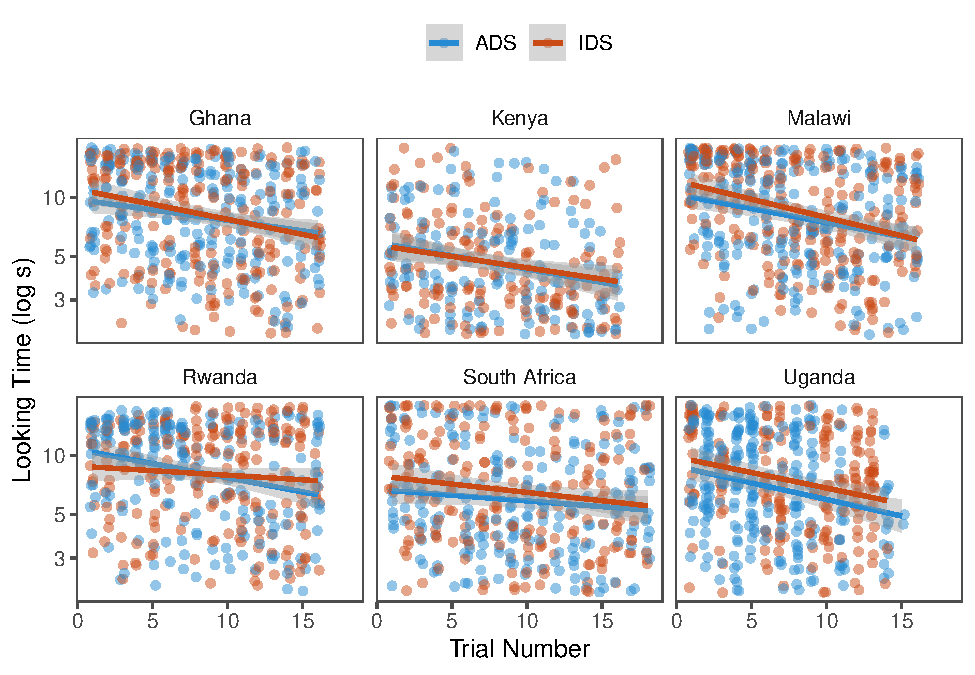
\includegraphics{mb1a-paper_files/figure-latex/unnamed-chunk-8-1.pdf}
\caption{\label{fig:unnamed-chunk-8}By lab results. Each dot represents one trial of looking time. X-axis represents the trial number. Y-axis represents the log looking time in seconds. Red represents IDS trials. Blue represents ADS trials.}
\end{figure}

\begin{table}

\caption{Model estimates for Research Questions 1 and 2. The baseline for trial type is adult-directed speech. Trial number is mean-centered. Age is measured in months and standardized.}
\centering
\begin{tabular}[t]{lcccc}
\toprule
Term & Estimate & std.error & t & p\\
\midrule
(Intercept) & 1.89 & 0.09 & 21.34 & < .01\\
Trial Type & 0.06 & 0.02 & 2.76 & 0.01\\
Trial Number & -0.03 & 0.00 & -9.72 & < .01\\
Age & -0.09 & 0.03 & -3.40 & < .01\\
Trial Type * Trial Number & 0.00 & 0.00 & -0.22 & 0.83\\
\addlinespace
Trial Number * Age & 0.00 & 0.00 & 1.60 & 0.11\\
Trial Type * Age & 0.02 & 0.02 & 0.94 & 0.35\\
\bottomrule
\end{tabular}
\end{table}

The model revealed a significant main effect of trial type, such that infants looked longer at IDS trials than ADS trials (Figure 1; Table 3; \emph{\(\beta\)} = 0.06; \emph{SE} = 0.02; \emph{t} = 2.76; \emph{p} = 0.01). There was also a significant negative effect of trial number, indicating that looking times decreased over the course of the session (\emph{\(\beta\)} = -0.03; \emph{SE} = 0; \emph{t} = -9.72; \emph{p} \textless{} 0.01). Age in months was also a significant predictor, with older infants showing shorter looking times overall (\emph{\(\beta\)} = -0.09; \emph{SE} = 0.03; \emph{t} = -3.40; \emph{p} \textless{} 0.01). None of the interaction terms reached statistical significance, including the interaction between trial type and age, suggesting that the magnitude of IDS preference did not change reliably with age.

Research question 3: Population comparison. In this analysis, we compare the data collected from the laboratories in Africa to data collected in MB1 and MB1B in Germany, Italy, New Zealand, Turkey, United Kingdom. We selected the subset of data from MB1 and MB1B that was collected using central fixation procedures (to match methods across studies) and from infants who were not exposed to North American English (non NAE) (to match stimulus un-familiarity due to language background). While we could have controlled the methodological and demographic variables statistically (and hence included all data from MB1 and MB1B in the full model), we believed that the increase in model complexity -- and comparable decrease in interpretability -- outweighed the benefits of this strategy.

We examine whether our sample of infants' IDS preference is different from those in MB1 and MB1B with the following model:
\texttt{log\_lt\ \textasciitilde{}\ trial\_type\ +\ trial\_num\ +\ age\_months\ +\ infant\_ID\ +\ language\_background\ +\ trial\_type\ *\ trial\_num\ +\ age\_months\ *\ trial\_num\ +\ age\_months\ *\ trial\_type\ +\ trial\_type\ *\ infant\_ID\ +\ trial\_num\ *\ infant\_ID\ +\ trial\_type\ *\ language\_background\ +\ (trial\_type\ *\ trial\_num\ \textbar{}\ subid)\ +\ (trial\_type\ \textbar{}\ lab)}

In this mixed-effects model, the fixed-effects included main effects of trial type, language background, age, trial number, infants in our study/non NAE infants in MB1(B) and language background. In addition, we included several two-way interaction terms in the fixed effects structure: (i) trial type interacted with trial number, modeling the possibility of infants' faster habituation to ADS, (ii) age interacted with trial number, modeling faster habituation for older children, (iii) age interacted with trial type, modeling the developmental trajectory of infants' IDS preference, (iv) trial type interacted with infants in our sample, modeling the possible difference in IDS preference between infants in Africa and infants tested in MB1 and MB1B, (v) trial num interacted with infants in our sample, modeling the possible difference in habituation between our sample of infants and infants tested in MB1 and MB1B, and (vi) trial type interacted with language background, modeling the possible difference in IDS preference from infants with different language backgrounds. We adopted the same baseline random effects as in the previous model.

After pruning for non-convergence, our final model specification was: \texttt{log\_lt\ \textasciitilde{}\ trial\_type\ +\ trial\_num\ +\ age\_months\ +\ infant\_ID\ +\ language\_background\ +\ trial\_type\ *\ trial\_num\ +\ age\_months\ *\ trial\_num\ +\ age\_months\ *\ trial\_type\ +\ trial\_type\ *\ infant\_ID\ +\ trial\_num\ *\ infant\_ID\ +\ trial\_type\ *\ language\_background\ +\ (1\ \textbar{}\ subid)\ +\ (1\ \textbar{}\ lab)}. The fixed effect estimate corresponding to our research question is the \texttt{trial\_type\ *\ infant\_ID}, which captures differences in measured IDS preference between the current data and data from MB1/MB1B in units of log seconds of looking time.

\begin{table}

\caption{Model estimates for Research Questions 3. The baseline for trial type is adult-directed speech (ADS), trial number is mean-centered, age is measured in months and standardized, the baseline for infant type is infants from MB1/MB1B (non-NAE sample), and the baseline for language background is bilingual infants.}
\centering
\begin{tabular}[t]{lcccc}
\toprule
Term & Estimate & SE & t & p\\
\midrule
(Intercept) & 1.77 & 0.07 & 24.16 & < .01\\
Trial Type & 0.02 & 0.03 & 0.66 & 0.51\\
Trial Number & -0.05 & 0.00 & -30.82 & < .01\\
Age & -0.13 & 0.02 & -8.38 & < .01\\
Infant Type & 0.15 & 0.12 & 1.32 & 0.21\\
\addlinespace
Language Background (Monolingual) & -0.02 & 0.05 & -0.48 & 0.63\\
Language Background (Other) & 0.02 & 0.07 & 0.24 & 0.81\\
Trial Type * Trial Number & 0.00 & 0.00 & -0.81 & 0.42\\
Trial Number * Age & -0.01 & 0.00 & -4.39 & < .01\\
Trial Type * Age & 0.02 & 0.01 & 1.86 & 0.06\\
\addlinespace
Trial Type * Infant Type & -0.01 & 0.03 & -0.26 & 0.80\\
Trial Number * Infant Type & 0.02 & 0.00 & 4.96 & <.01\\
Trial Type * Language Background (Monolingual) & 0.04 & 0.03 & 1.42 & 0.16\\
Trial Type * Language Background (Other) & 0.00 & 0.05 & 0.07 & 0.95\\
\bottomrule
\end{tabular}
\end{table}

The model revealed no significant difference in IDS preference between infants tested in our sample and those tested in MB1/MB1B, as indicated by the non-significant interaction between trial type and infant group (Table 4; \emph{\(\beta\)} = -0.01; \emph{SE} = 0.03; \emph{t} = -0.26; \emph{p} = 0.80). However, there was a significant main effect of trial type (\emph{\(\beta\)} = 0.02; \emph{SE} = 0.03; \emph{t} = 0.66; \emph{p} = 0.51), suggesting that infants showed a reliable preference to IDS over ADS.

Consistent with expectations, looking times decreased over the course of the session (\emph{\(\beta\)} = -0.05; \emph{SE} = 0; \emph{t} = -30.82; \emph{p} \textless{} 0.01), and older infants looked for less time overall (\emph{\(\beta\)} = -0.13; \emph{SE} = 0.02; \emph{t} = -8.38; p \textless{} .001). We also found that older infants habituated more quickly, as indicated by a significant negative interaction between age and trial number (\emph{\(\beta\)} = -0.01; \emph{SE} = 0; \emph{t} = -4.39; p \textless{} .001). The interaction between trial number and infant group was also significant (\emph{\(\beta\)} = 0.02; \emph{SE} = 0; \emph{t} = 4.96; p \textless{} .001), indicating that looking times declined more slowly across trials for infants in our sample compared to those in MB1/MB1B. No other interactions reached significance.

\hypertarget{exploratory-analyses}{%
\subsection{Exploratory Analyses}\label{exploratory-analyses}}

SES. Previous research in North America (e.g., Hart \& Risley, 1995; Hoff, 2006b; Weisleder \& Fernald, 2013) has shown that the quantity and quality of child-directed speech vary across families with different SES backgrounds. These differences in language input may drive differences in infants' preference for IDS. Thus, we explored how SES affects infants' preference for IDS. SES was measured by primary caregiver's formal education (number of years). We entered primary caregiver's formal education (in years) as a predictor in the regression model specified for RQ1 and RQ2, along with its interaction with trial type.

The interaction between trial type and primary caregiver education was not significant (\emph{\(\beta\)} = -0.01; \emph{SE} = 0.02; \emph{t} = -0.46; \emph{p} = 0.65), not allowing rejection of the null hypothesis that SES does not moderate infants' preference for IDS. In other words, the magnitude of IDS preference was similar regardless of caregivers' years of formal education. At the same time, we did observe a significant main effect of trial type, with infants looking longer at IDS than ADS trials overall (\emph{\(\beta\)} = 0.06; \emph{SE} = 0.02; \emph{t} = 2.55; \emph{p} = 0.01). Looking times decreased significantly across trials (\emph{\(\beta\)} = -0.04; \emph{SE} = 0; \emph{t} = -9.92; \emph{p} \textless{} 0.01), and older infants looked for less time overall (\emph{\(\beta\)} = -0.04; \emph{SE} = 0; \emph{t} = -9.92; \emph{p} \textless{} 0.01). No other interactions were significant. As a robustness check, we re-ran the model on the subset of infants with female primary caregivers (80.52\% infants). The pattern of results was qualitatively unchanged.

Meta-analysis. For comparison with ManyBabies 1 and 1B, we computed standardized effect sizes for each lab following the method used in ManyBabies Consortium (2020). The resulting meta-analytic plot is shown in Appendix B: Figure B1. The meta-analytic effect size is 0.17{[}-0.03, 0.37{]}, which is numerically smaller than the .35 {[}0.29, 0.42{]} reported in MB1 (Manybabies Consortium, 2020) but these estimates are not directly comparable due to the different method and age distribution in the current project (cf., Zettersten et al., 2024).

\hypertarget{general-discussion}{%
\section{General Discussion}\label{general-discussion}}

Infants' preference for IDS is both an important phenomenon for understanding language learning and a case study for infant methods more broadly. The MB1 study investigated variation in IDS preference across laboratories and across countries and found a small but reliable effect such that infants preferred IDS over ADS; though there was substantial variation across labs, much of this variation was in fact due to sampling variation. Nevertheless, the effect was moderated by infant age, language background, and experimental method. Though MB1 and its sister project MB1B investigated children from a wide variety of language backgrounds, no sites from Africa were included in this initial group of participating laboratories. The current study was designed to fill this gap.

We summarize our findings with respect to three research questions in the paper. First, consistent with MB1 and MB1B, we found evidence for a significant IDS preference in a sample of 200 African infants. Second, and unlike MB1, we did not find significant age-related variation in IDS preference, but given the relatively small magnitude of the overall effect, we may not have had sufficient power to detect an interaction with age in our primary analytic model. In addition, the variability in age across sites was limited, with four of the six labs having mean ages clustered around 8 to 9 months, leaving us little age variation to detect such an effect.

Finally, we were interested in comparing the magnitude of the IDS preference in the current study to the estimates obtained in MB1 and MB1B (with multilingual data providing an important comparison because of the diverse language backgrounds in our current sample). We did not find significant study effects in a model comparing data from the current study to a method- and language-background matched sample of infants from MB1 and MB1B. The magnitude of the IDS preference in African infants in the current study (\(d = 0.17\)) was numerically smaller than the overall estimate reported by MB1 (\(d = 0.35\)), but the two estimates are not directly comparable; among other things, the current study was conducted with infants who were not growing up learning North American English and it used the central fixation method, both of which were associated with overall lower effect sizes in MB1 compared with other groups (Zettersten et al., 2024).

The current study provides important evidence on the generalizability of the IDS preference and of looking-time methods in infancy more broadly. Despite the diversity of MB1, as noted above, the vast majority of labs were from Western countries where Indo-European languages are spoken. Thus, the findings of the current study provide evidence that the IDS preference observed in MB1 is present in infants growing up in a diverse array of non-WEIRD environments. More broadly, there is limited work using looking time methods for infancy research in the African context (cf. Pyykkö et al., 2019), so our findings also serve as an important datapoint demonstrating the generality of these techniques for children worldwide.

A second goal of the current study was to build a team of laboratories in Africa collecting data with infants. We were successful in accomplishing this goal and we believe that the current study represents the largest experimental study of African infants to date. Despite this success, we encountered a number of substantial challenges. Some of these were unique to the African context and to the specific time-period of our study (e.g., spanning the Covid-19 pandemic) while others were more general to the project of conducting ``big team science'' investigations across institutions with a wide range of resources.

Although we received commitments for data collection from 11 teams, three of these teams were unable to collect data due to a variety of challenges relating to personnel and resources. One source of these challenges was the initiation of Covid-19 lockdowns soon after our initial project training in the winter of 2020. In some cases, personnel left the project or priorities changed, leading teams to lose the ability to participate. These lockdowns were also difficult even for teams who stayed involved in the project. Due to turnover and the long delay between initial training and setup for data collection after restrictions were eased, a number of procedural deviations were introduced. In two cases, these deviations were so severe that we could not analyze data from the site. In an ideal world, our group would have been able to conduct additional site visits and training after sites began collecting data; unfortunately this was not possible due to budget and personnel limitations.

The current study has a number of further scientific limitations, including some shared with prior studies including MB1 and MB1B. First, although we attempted to estimate IDS preference, we did so using a specific set of speech stimuli and a specific paradigm. It is likely that the stimuli used here are less extreme than many used in prior studies, and further, they are produced in North American English, making them linguistically unfamiliar to one degree or another to all of the infants in our study. Followups using native language stimuli are needed to measure the importance of this choice to the IDS preference. Second, although we invited broad participation, our samples are convenience samples in at least two ways: both of the sites who participated and the infants who participated at each site. Thus our effect size estimates cannot be treated as population effects but rather ``proof of concept'' that an IDS preference can be observed in African infants across a diverse set of sites. Finally, although we did not observe major demographic variation, we caution against over-interpretation of any demographic differences in IDS preference given that IDS preference has not been shown to be individually predictive of any later outcomes (Soderstrom et al., 2024).

In sum, our study offers a case study of ``big team science'' (Coles, Hamlin, Sullivan, Parker, \& Altschul, 2022) carried out via a collaboration between African researchers and the ManyBabies Consortium. Although it faced a variety of logistical challenges (many shared with other grass roots efforts; Baumgartner et al., 2023), it nevertheless yields important evidence on generalizability, of a key phenomenon in early language learning, of looking time methods, and finally of a broad-based collaborative model for studying infant development.

\newpage

\hypertarget{references}{%
\section{References}\label{references}}

\begingroup
\setlength{\parindent}{-0.5in}
\setlength{\leftskip}{0.5in}

\hypertarget{refs}{}
\begin{CSLReferences}{1}{0}
\leavevmode\vadjust pre{\hypertarget{ref-barr2013a}{}}%
Barr, D. J., Levy, R., Scheepers, C., \& Tily, H. J. (2013). Random effects structure for confirmatory hypothesis testing: Keep it maximal. \emph{Journal of Memory and Language}, \emph{68}(3), 255--278. \url{https://doi.org/10.1016/j.jml.2012.11.001}

\leavevmode\vadjust pre{\hypertarget{ref-bates2015}{}}%
Bates, D., Mächler, M., Bolker, B., \& Walker, S. (2015). Fitting linear mixed-effects models using lme4. \emph{Journal of Statistical Software}, \emph{67}(1). \url{https://doi.org/10.18637/jss.v067.i01}

\leavevmode\vadjust pre{\hypertarget{ref-baumgartner2023build}{}}%
Baumgartner, H. A., Alessandroni, N., Byers-Heinlein, K., Frank, M. C., Hamlin, J. K., Soderstrom, M., \ldots{} Coles, N. A. (2023). How to build up big team science: A practical guide for large-scale collaborations. \emph{Royal Society Open Science}, \emph{10}(6), 230235.

\leavevmode\vadjust pre{\hypertarget{ref-broesch2015b}{}}%
Broesch, T. L., \& Bryant, G. A. (2015). Prosody in infant-directed speech is similar across western and traditional cultures. \emph{Journal of Cognition and Development}, \emph{16}(1), 31--43. \url{https://doi.org/10.1080/15248372.2013.833923}

\leavevmode\vadjust pre{\hypertarget{ref-bryant2007recognizing}{}}%
Bryant, G. A., \& Barrett, H. C. (2007). Recognizing intentions in infant-directed speech: Evidence for universals. \emph{Psychological Science}, \emph{18}(8), 746--751.

\leavevmode\vadjust pre{\hypertarget{ref-bryant2012recognizing}{}}%
Bryant, G. A., Liénard, P., \& Clark Barrett, H. (2012). Recognizing infant-directed speech across distant cultures: Evidence from africa. \emph{Journal of Evolutionary Psychology}, \emph{10}(2), 47--59.

\leavevmode\vadjust pre{\hypertarget{ref-byers2021multilab}{}}%
Byers-Heinlein, K., Tsui, A. S. M., Bergmann, C., Black, A. K., Brown, A., Carbajal, M. J., et al.others. (2021). A multilab study of bilingual infants: Exploring the preference for infant-directed speech. \emph{Advances in Methods and Practices in Psychological Science}, \emph{4}(1), 2515245920974622.

\leavevmode\vadjust pre{\hypertarget{ref-casillas2020}{}}%
Casillas, M., Brown, P., \& Levinson, S. C. (2020). Early language experience in a tseltal mayan village. \emph{Child Development}, \emph{91}(5), 1819--1835. \url{https://doi.org/10.1111/cdev.13349}

\leavevmode\vadjust pre{\hypertarget{ref-casillas2021}{}}%
Casillas, M., Brown, P., \& Levinson, S. C. (2021). Early language experience in a papuan community. \emph{Journal of Child Language}, \emph{48}(4), 792--814. \url{https://doi.org/10.1017/S0305000920000549}

\leavevmode\vadjust pre{\hypertarget{ref-coles2022build}{}}%
Coles, N. A., Hamlin, J. K., Sullivan, L. L., Parker, T. H., \& Altschul, D. (2022). Build up big-team science. \emph{Nature}, \emph{601}(7894), 505--507.

\leavevmode\vadjust pre{\hypertarget{ref-manybabies2020quantifying}{}}%
Consortium, M. (2020). Quantifying sources of variability in infancy research using the infant-directed-speech preference. \emph{Advances in Methods and Practices in Psychological Science}, \emph{3}(1), 24--52.

\leavevmode\vadjust pre{\hypertarget{ref-cooper1997}{}}%
Cooper, R. P., Abraham, J., Berman, S., \& Staska, M. (1997). The development of infants' preference for motherese. \emph{Infant Behavior and Development}, \emph{20}(4), 477--488. \url{https://doi.org/10.1016/S0163-6383(97)90037-0}

\leavevmode\vadjust pre{\hypertarget{ref-cooper1990}{}}%
Cooper, R. P., \& Aslin, R. N. (1990). Preference for infant-directed speech in the first month after birth. \emph{Child Development}, \emph{61}(5), 1584--1595. \url{https://doi.org/10.2307/1130766}

\leavevmode\vadjust pre{\hypertarget{ref-cooper1994}{}}%
Cooper, R. P., \& Aslin, R. N. (1994). Developmental differences in infant attention to the spectral properties of infant-directed speech. \emph{Child Development}, \emph{65}(6), 1663--1677. \url{https://doi.org/10.2307/1131286}

\leavevmode\vadjust pre{\hypertarget{ref-cristia2019child}{}}%
Cristia, A., Dupoux, E., Gurven, M., \& Stieglitz, J. (2019). Child-directed speech is infrequent in a forager-farmer population: A time allocation study. \emph{Child Development}, \emph{90}(3), 759--773.

\leavevmode\vadjust pre{\hypertarget{ref-csibra2016}{}}%
Csibra, G., Hernik, M., Mascaro, O., Tatone, D., \& Lengyel, M. (2016). Statistical treatment of looking-time data. \emph{Developmental Psychology}, \emph{52}(4), 521--536. \url{https://doi.org/10.1037/dev0000083}

\leavevmode\vadjust pre{\hypertarget{ref-dunst2012preference}{}}%
Dunst, C., Gorman, E., \& Hamby, D. (2012). Preference for infant-directed speech in preverbal young children. \emph{Center for Early Literacy Learning}, \emph{5}(1), 1--13.

\leavevmode\vadjust pre{\hypertarget{ref-farran2016cross}{}}%
Farran, L. K., Lee, C.-C., Yoo, H., \& Oller, D. K. (2016). Cross-cultural register differences in infant-directed speech: An initial study. \emph{PloS One}, \emph{11}(3), e0151518.

\leavevmode\vadjust pre{\hypertarget{ref-fernald1985}{}}%
Fernald, A. (1985). Four-month-old infants prefer to listen to motherese. \emph{Infant Behavior and Development}, \emph{8}(2), 181--195. \url{https://doi.org/10.1016/S0163-6383(85)80005-9}

\leavevmode\vadjust pre{\hypertarget{ref-fernald1989}{}}%
Fernald, A., Taeschner, T., Dunn, J., Papousek, M., Boysson-Bardies, B. de, \& Fukui, I. (1989). A cross-language study of prosodic modifications in mothers' and fathers' speech to preverbal infants. \emph{Journal of Child Language}, \emph{16}(3), 477--501. \url{https://doi.org/10.1017/S0305000900010679}

\leavevmode\vadjust pre{\hypertarget{ref-frank2017}{}}%
Frank, M. C., Bergelson, E., Bergmann, C., Cristia, A., Floccia, C., Gervain, J., \ldots{} Yurovsky, D. (2017). A collaborative approach to infant research: Promoting reproducibility, best practices, and theory-building. \emph{Infancy}, \emph{22}(4), 421--435. \url{https://doi.org/10.1111/infa.12182}

\leavevmode\vadjust pre{\hypertarget{ref-grafestes2013}{}}%
Graf Estes, K., \& Hurley, K. (2013). Infant-directed prosody helps infants map sounds to meanings. \emph{Infancy}, \emph{18}(5), 797--824. \url{https://doi.org/10.1111/infa.12006}

\leavevmode\vadjust pre{\hypertarget{ref-grieser1988maternal}{}}%
Grieser, D. L., \& Kuhl, P. K. (1988). Maternal speech to infants in a tonal language: Support for universal prosodic features in motherese. \emph{Developmental Psychology}, \emph{24}(1), 14.

\leavevmode\vadjust pre{\hypertarget{ref-hart1995}{}}%
Hart, B., \& Risley, T. R. (1995). \emph{Meaningful differences in the everyday experience of young american children}. P.H. Brookes.

\leavevmode\vadjust pre{\hypertarget{ref-hayashi2001}{}}%
Hayashi, A., Tamekawa, Y., \& Kiritani, S. (2001). Developmental change in auditory preferences for speech stimuli in japanese infants. \emph{Journal of Speech, Language, and Hearing Research}, \emph{44}(6), 1189--1200. \url{https://doi.org/10.1044/1092-4388(2001/092)}

\leavevmode\vadjust pre{\hypertarget{ref-heath1983}{}}%
Heath, S. B. (1983). \emph{Ways with words: Language, life, and work in communities and classrooms}. Cambridge University Press.

\leavevmode\vadjust pre{\hypertarget{ref-henrich2010weirdest}{}}%
Henrich, J., Heine, S. J., \& Norenzayan, A. (2010). The weirdest people in the world? \emph{Behavioral and Brain Sciences}, \emph{33}(2-3), 61--83.

\leavevmode\vadjust pre{\hypertarget{ref-hoff2006social}{}}%
Hoff, E. (2006b). How social contexts support and shape language development. \emph{Developmental Review}, \emph{26}(1), 55--88.

\leavevmode\vadjust pre{\hypertarget{ref-hoff2006}{}}%
Hoff, E. (2006a). How social contexts support and shape language development. \emph{Developmental Review}, \emph{26}(1), 55--88. \url{https://doi.org/10.1016/j.dr.2005.11.002}

\leavevmode\vadjust pre{\hypertarget{ref-huttenlocher2010sources}{}}%
Huttenlocher, J., Waterfall, H., Vasilyeva, M., Vevea, J., \& Hedges, L. V. (2010). Sources of variability in children's language growth. \emph{Cognitive Psychology}, \emph{61}(4), 343--365.

\leavevmode\vadjust pre{\hypertarget{ref-keller2012}{}}%
Keller, H. (2012). Autonomy and relatedness revisited: Cultural manifestations of universal human needs. \emph{Child Development Perspectives}, \emph{6}(1), 12--18. \url{https://doi.org/10.1111/j.1750-8606.2011.00208.x}

\leavevmode\vadjust pre{\hypertarget{ref-kitamura2009}{}}%
Kitamura, C., \& Lam, C. (2009). Age-specific preferences for infant-directed affective intent. \emph{Infancy}, \emph{14}(1), 77--100. \url{https://doi.org/10.1080/15250000802569777}

\leavevmode\vadjust pre{\hypertarget{ref-kitamura2001universality}{}}%
Kitamura, C., Thanavishuth, C., Burnham, D., \& Luksaneeyanawin, S. (2001). Universality and specificity in infant-directed speech: Pitch modifications as a function of infant age and sex in a tonal and non-tonal language. \emph{Infant Behavior and Development}, \emph{24}(4), 372--392.

\leavevmode\vadjust pre{\hypertarget{ref-koo2016guideline}{}}%
Koo, T. K., \& Li, M. Y. (2016). A guideline of selecting and reporting intraclass correlation coefficients for reliability research. \emph{Journal of Chiropractic Medicine}, \emph{15}(2), 155--163.

\leavevmode\vadjust pre{\hypertarget{ref-kuznetsova2017}{}}%
Kuznetsova, A., Brockhoff, P. B., \& Christensen, R. H. B. (2017). lmerTest package: Tests in linear mixed effects models. \emph{Journal of Statistical Software}, \emph{82}(13). \url{https://doi.org/10.18637/jss.v082.i13}

\leavevmode\vadjust pre{\hypertarget{ref-legare2019development}{}}%
Legare, C. H. (2019). The development of cumulative cultural learning. \emph{Annual Review of Developmental Psychology}, \emph{1}(1), 119--147.

\leavevmode\vadjust pre{\hypertarget{ref-levine1994}{}}%
LeVine, R. A. (Ed.). (1994). \emph{Child care and culture: Lessons from africa} (Reprinted). Cambridge University Press.

\leavevmode\vadjust pre{\hypertarget{ref-levine2016}{}}%
LeVine, R. A., \& LeVine, S. (2016). \emph{Do parents matter? Why japanese babies sleep well, mexican siblings don't fight, and american parents should just relax} (First). PublicAffairs.

\leavevmode\vadjust pre{\hypertarget{ref-mathur2020robust}{}}%
Mathur, M. B., \& VanderWeele, T. J. (2020). Robust metrics and sensitivity analyses for meta-analyses of heterogeneous effects. \emph{Epidemiology}, \emph{31}(3), 356--358.

\leavevmode\vadjust pre{\hypertarget{ref-newman2006}{}}%
Newman, R. S., \& Hussain, I. (2006). Changes in preference for infant-directed speech in low and moderate noise by 4.5- to 13-month-olds. \emph{Infancy}, \emph{10}(1), 61--76. \url{https://doi.org/10.1207/s15327078in1001_4}

\leavevmode\vadjust pre{\hypertarget{ref-nielsen2017}{}}%
Nielsen, M., Haun, D., Kärtner, J., \& Legare, C. H. (2017). The persistent sampling bias in developmental psychology: A call to action. \emph{Journal of Experimental Child Psychology}, \emph{162}, 31--38. \url{https://doi.org/10.1016/j.jecp.2017.04.017}

\leavevmode\vadjust pre{\hypertarget{ref-openscience2015}{}}%
Open Science Collaboration. (2015). Estimating the reproducibility of psychological science. \emph{Science}, \emph{349}(6251), aac4716. \url{https://doi.org/10.1126/science.aac4716}

\leavevmode\vadjust pre{\hypertarget{ref-parsons2019psychological}{}}%
Parsons, S., Kruijt, A.-W., \& Fox, E. (2019). Psychological science needs a standard practice of reporting the reliability of cognitive-behavioral measurements. \emph{Advances in Methods and Practices in Psychological Science}, \emph{2}(4), 378--395.

\leavevmode\vadjust pre{\hypertarget{ref-pegg1992}{}}%
Pegg, J. E., Werker, J. F., \& McLeod, P. J. (1992). Preference for infant-directed over adult-directed speech: Evidence from 7-week-old infants. \emph{Infant Behavior and Development}, \emph{15}(3), 325--345. \url{https://doi.org/10.1016/0163-6383(92)80003-D}

\leavevmode\vadjust pre{\hypertarget{ref-posel2016}{}}%
Posel, D., \& Zeller, J. (2016). Language shift or increased bilingualism in south africa: Evidence from census data. \emph{Journal of Multilingual and Multicultural Development}, \emph{37}(4), 357--370. \url{https://doi.org/10.1080/01434632.2015.1072206}

\leavevmode\vadjust pre{\hypertarget{ref-pyykko2019early}{}}%
Pyykkö, J., Forssman, L., Maleta, K., Ashorn, P., Ashorn, U., \& Leppänen, J. M. (2019). Early development of visual attention in infants in rural malawi. \emph{Developmental Science}, \emph{22}(5), e12761.

\leavevmode\vadjust pre{\hypertarget{ref-ramirez2014}{}}%
Ramı́rez-Esparza, N., Garcı́a-Sierra, A., \& Kuhl, P. K. (2014). Look who's talking: Speech style and social context in language input to infants are linked to concurrent and future speech development. \emph{Developmental Science}, \emph{17}(6), 880--891. \url{https://doi.org/10.1111/desc.12172}

\leavevmode\vadjust pre{\hypertarget{ref-revelle2017psych}{}}%
Revelle, W. R. (2017). \emph{Psych: Procedures for personality and psychological research}.

\leavevmode\vadjust pre{\hypertarget{ref-rosenhouse2004}{}}%
Rosenhouse, J., \& Goral, M. (2004). 31 bilingualism in the middle east and north africa: A focus on the arabic-speaking world. \emph{The Handbook of Bilingualism}, 835.

\leavevmode\vadjust pre{\hypertarget{ref-rowe2012longitudinal}{}}%
Rowe, M. L. (2012). A longitudinal investigation of the role of quantity and quality of child-directed speech in vocabulary development. \emph{Child Development}, \emph{83}(5), 1762--1774.

\leavevmode\vadjust pre{\hypertarget{ref-santesso2007frontal}{}}%
Santesso, D. L., Schmidt, L. A., \& Trainor, L. J. (2007). Frontal brain electrical activity (EEG) and heart rate in response to affective infant-directed (ID) speech in 9-month-old infants. \emph{Brain and Cognition}, \emph{65}(1), 14--21.

\leavevmode\vadjust pre{\hypertarget{ref-schneidman2012}{}}%
Schneidman, L. A., \& Goldin-Meadow, S. (2012). Language input and acquisition in a mayan village: How important is directed speech? \emph{Developmental Science}, \emph{15}(5), 659--673. \url{https://doi.org/10.1111/j.1467-7687.2012.01168.x}

\leavevmode\vadjust pre{\hypertarget{ref-schreiner2024limited}{}}%
Schreiner, M. S., Zettersten, M., Bergmann, C., Frank, M. C., Fritzsche, T., Gonzalez-Gomez, N., et al.others. (2024). Limited evidence of test-retest reliability in infant-directed speech preference in a large preregistered infant experiment. \emph{Developmental Science}, \emph{27}(6), e13551.

\leavevmode\vadjust pre{\hypertarget{ref-shneidman2012language}{}}%
Shneidman, L. A., \& Goldin-Meadow, S. (2012). Language input and acquisition in a mayan village: How important is directed speech? \emph{Developmental Science}, \emph{15}(5), 659--673.

\leavevmode\vadjust pre{\hypertarget{ref-shneidman2013}{}}%
Shneidman, L., Arroyo, M., Levine, S. C., \& Goldin-Meadow, S. (2013). What counts as effective input for word learning? \emph{Developmental Science}, \emph{16}(6), 993--1009. \url{https://doi.org/10.1111/desc.12055}

\leavevmode\vadjust pre{\hypertarget{ref-singh2002}{}}%
Singh, L., Morgan, J. L., \& Best, C. T. (2002). Infants' listening preferences: Baby talk or happy talk? \emph{Infancy}, \emph{3}(3), 365--394. \url{https://doi.org/10.1207/S15327078IN0303_5}

\leavevmode\vadjust pre{\hypertarget{ref-singh2009influences}{}}%
Singh, L., Nestor, S., Parikh, C., \& Yull, A. (2009). Influences of infant-directed speech on early word recognition. \emph{Infancy}, \emph{14}(6), 654--666.

\leavevmode\vadjust pre{\hypertarget{ref-soderstrom2024testing}{}}%
Soderstrom, M., Rocha-Hidalgo, J., Muñoz, L. E., Bochynska, A., Werker, J. F., Skarabela, B., et al.others. (2024). Testing the relationship between preferences for infant-directed speech and vocabulary development: A multi-lab study. \emph{Journal of Child Language}, 1--26.

\leavevmode\vadjust pre{\hypertarget{ref-thiessen2005infant}{}}%
Thiessen, E. D., Hill, E. A., \& Saffran, J. R. (2005). Infant-directed speech facilitates word segmentation. \emph{Infancy}, \emph{7}(1), 53--71.

\leavevmode\vadjust pre{\hypertarget{ref-trainor2002pitch}{}}%
Trainor, L. J., \& Desjardins, R. N. (2002). Pitch characteristics of infant-directed speech affect infants' ability to discriminate vowels. \emph{Psychonomic Bulletin \& Review}, \emph{9}(2), 335--340.

\leavevmode\vadjust pre{\hypertarget{ref-vogt2015communicative}{}}%
Vogt, P., Mastin, J. D., \& Schots, D. M. (2015). Communicative intentions of child-directed speech in three different learning environments: Observations from the netherlands, and rural and urban mozambique. \emph{First Language}, \emph{35}(4-5), 341--358.

\leavevmode\vadjust pre{\hypertarget{ref-weber2017cultural}{}}%
Weber, A., Fernald, A., \& Diop, Y. (2017). When cultural norms discourage talking to babies: Effectiveness of a parenting program in rural senegal. \emph{Child Development}, \emph{88}(5), 1513--1526.

\leavevmode\vadjust pre{\hypertarget{ref-weisleder2013talking}{}}%
Weisleder, A., \& Fernald, A. (2013). Talking to children matters: Early language experience strengthens processing and builds vocabulary. \emph{Psychological Science}, \emph{24}(11), 2143--2152.

\leavevmode\vadjust pre{\hypertarget{ref-werker1989infant}{}}%
Werker, J. F., \& McLeod, P. J. (1989). Infant preference for both male and female infant-directed talk: A developmental study of attentional and affective responsiveness. \emph{Canadian Journal of Psychology/Revue Canadienne de Psychologie}, \emph{43}(2), 230.

\leavevmode\vadjust pre{\hypertarget{ref-werker1994cross}{}}%
Werker, J. F., Pegg, J. E., \& McLeod, P. J. (1994). A cross-language investigation of infant preference for infant-directed communication. \emph{Infant Behavior and Development}, \emph{17}(3), 323--333.

\leavevmode\vadjust pre{\hypertarget{ref-zettersten2024evidence}{}}%
Zettersten, M., Cox, C., Bergmann, C., Tsui, A. S. M., Soderstrom, M., Mayor, J., et al.others. (2024). Evidence for infant-directed speech preference is consistent across large-scale, multi-site replication and meta-analysis. \emph{Open Mind}, \emph{8}, 439--461.

\end{CSLReferences}

\endgroup

\newpage

\newpage

\hypertarget{appendix-appendix}{%
\appendix}


\hypertarget{discrepancies-between-pre-registration-and-final-analyses}{%
\section{Discrepancies between pre-registration and final analyses}\label{discrepancies-between-pre-registration-and-final-analyses}}

\begin{enumerate}
\def\labelenumi{\arabic{enumi}.}
\item
  \textbf{ICC comparison}\\
  \emph{Pre-registration:} We planned to compare the estimated ICC in our study with the ICC reported in MB1(B).

  \emph{Final:} This comparison was not conducted because MB1(B) did not report ICC values.
\item
  \textbf{Metrics of effect heterogeneity}\\
  \emph{Pre-registration:} We planned to report distributional metrics describing heterogeneity across labs (Mathur \& VanderWeele, 2020) using the \emph{MetaUtility} package. Specifically, we proposed to estimate: (1) the percentage of effects greater than 0, (2) the percentage greater than Cohen's d = 0.2, and (3) the percentage less than d = --0.2. These metrics were to be reported only if random slopes of trial type by lab were included in the final model, their variance was estimated as greater than 0, and at least 10 labs contributed data.\\
  \emph{Final:} Random slopes of trial type by lab were not included in the final model, and only six labs contributed data. As a result, we did not estimate these metrics.
\item
  \textbf{Subset of MB1 and MB1(B) data}\\
  \emph{Pre-registration:} We planned to subset MB1 and MB1(B) data to include only infants tested with central fixation procedures and infants not exposed to North American English (NAE), to maximize comparability with the present study.\\
  \emph{Final:} In MB1 and MB1(B) data, information about English exposure often did not distinguish between American and British English. Therefore, we excluded infants based on country of residence (United States/Canada) rather than reported language exposure.
\item
  \textbf{Urban--rural exploratory analysis}\\
  \emph{Pre-registration:} We planned an exploratory analysis testing whether infants' IDS preference differed between urban and rural areas, motivated by prior findings of differences in parental speech input across these contexts (e.g., Keller, 2012; Vogt et al., 2015).
  \emph{Final:} We did not collect information on urban versus rural residence, so this analysis was not conducted.
\item
  \textbf{Socioeconomic status (SES) analyses}\\
  \emph{Pre-registration:} We planned to measure SES using both mothers' years of formal education and the MacArthur Scale of Subjective Social Status (MacSSS), including both variables in regression models.\\
  \emph{Final:} We did not have MacSSS data for most participants, and information on mothers' education was incomplete. We therefore used primary caregiver education as the main SES variable and conducted a robustness check using the subset of infant whose primary caregiver's sex is female.
\end{enumerate}

\hypertarget{by-lab-meta-analysis}{%
\section{By-lab Meta-analysis}\label{by-lab-meta-analysis}}

We computed a single effect size per lab and fit an intercept-only mixed-effect meta-regression to estimate the overall IDS preference across sites.This approach provides a comparable summary of results across sites. Even with a standardized protocol, sites differ in their cultures, recruitment pools, equipment, and experimenter behavior. A random-effects meta-analysis treats those differences as legitimate heterogeneity rather than noise, yielding a conservative estimate of the cross-lab mean and its uncertainty.

To do so, we calculated each infant's mean IDS--ADS difference score \footnote{ Due to an experimental procedure error, infants at the South Africa site were not always presented with complete IDS--ADS stimulus pairs; in some cases, the same stimulus was played multiple times. While this issue did not affect the random-effects model in the main analysis, it does impact the present meta-analysis. We therefore trimmed the data by (1) retaining only the first presentation of each trial and (2) including only trials in which both the IDS and ADS versions were presented. The trimmed data includes 176 trials from 28 infants.}, standardized these within lab to obtain, and estimated their sampling variances. These lab-level estimates were then entered into a REML random-effects model to produce the pooled effect size and 95\% confidence interval (Figure 1). The meta-analytic effect size is 0.17{[}-0.03, 0.37{]}, which is numerically smaller than the .35 {[}0.29, 0.42{]} reported in MB1 (Manybabies Consortium, 2020) but these estimates are not directly comparable due to the different method and age distribution in the current project (cf.~Mathur et al., 2024).

\begin{figure}
\centering
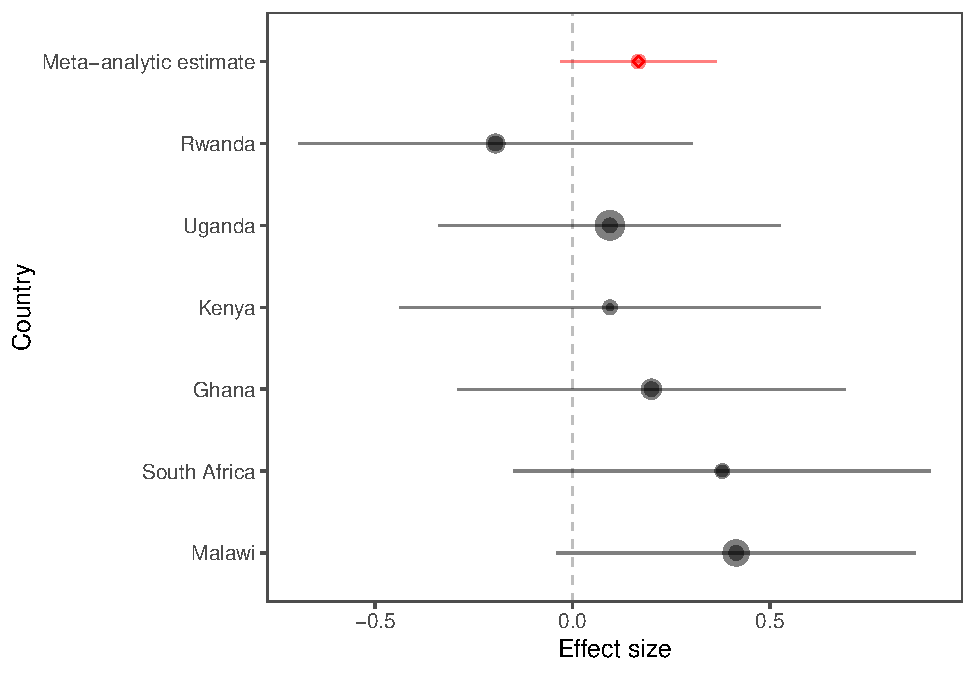
\includegraphics{mb1a-paper_files/figure-latex/unnamed-chunk-35-1.pdf}
\caption{\label{fig:unnamed-chunk-35}Forest plot of lab-level standardized effect sizes (for the IDS--ADS preference. Points represent individual country estimates, with size proportional to the inverse of their sampling variance; horizontal bars show 95\% confidence intervals. The meta-analytic aggregate (top, red) is from an intercept-only random-effects model.}
\end{figure}


\end{document}
